\documentclass[10pt,a4paper]{article}
\usepackage[margin=18mm]{geometry}\usepackage{fontspec,amsmath,graphicx,booktabs}
\setmainfont{Latin Modern Roman}\setlength{\parindent}{0pt}\setlength{\parskip}{6pt}
\begin{document}
{\LARGE More complex background and inverse-circle tests}\par 6 October 2026

\textbf{Main findings.} Adding bounded interference modestly improves the equal-arc intensity fit but leaves the inner-loop discrepancy. Direct signal inversion and circle fitting is computationally possible, and a known synthetic cone is recovered to numerical precision. Circle residual alone, however, admits a collapse/cancellation solution. A constrained inverse reconstruction remains an exploratory branch-specific test, not a validated replacement.

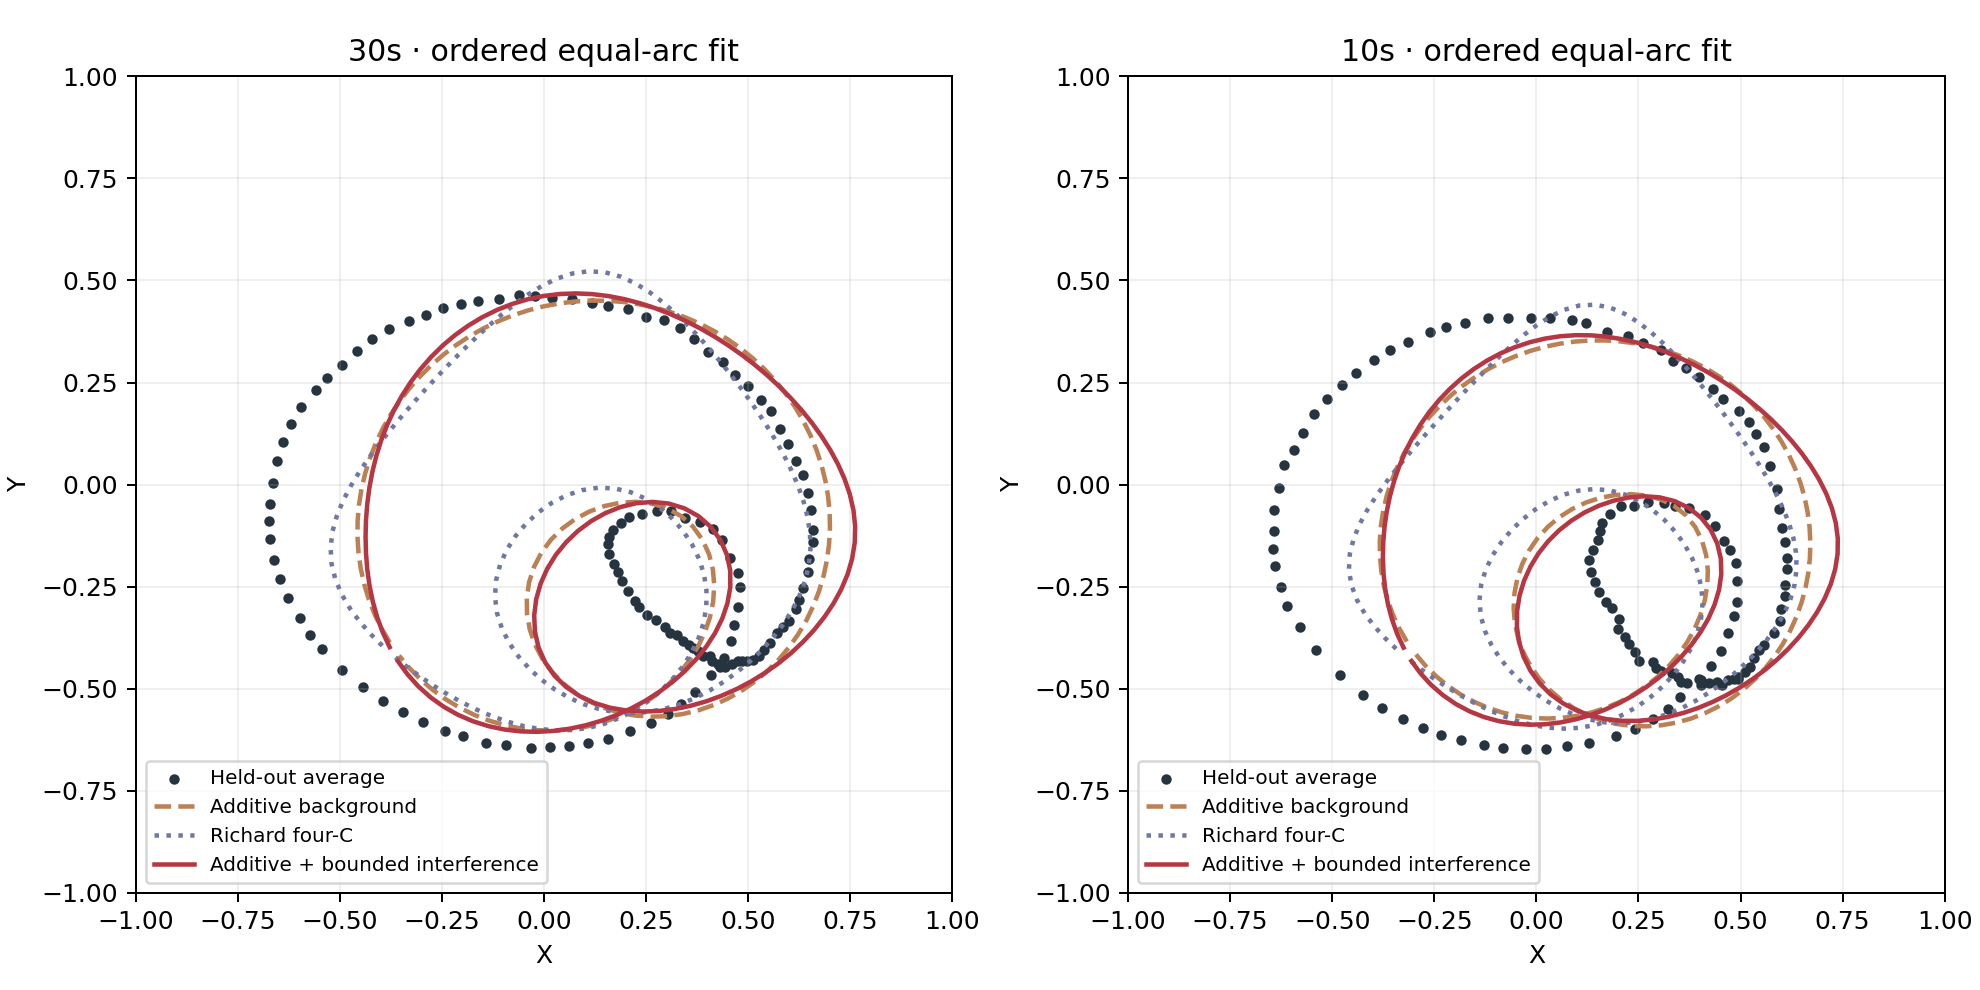
\includegraphics[width=\linewidth]{complex_arc.png}

\begin{tabular}{llrrrr}\toprule
Window & Equal-arc model & Channel RMS & XY RMS & BG/\(T_{\max}\) & \(\theta\) range\\\midrule
30s & Additive & 0.02990 & 0.14642 & 34.1\% & 37.8--90.0$^\circ$ \\
30s & Richard four-C & 0.03641 & 0.16645 & --- & 36.6--74.6$^\circ$ \\
30s & Additive + interference & 0.02780 & 0.14591 & 32.4\% & 38.2--90.0$^\circ$ \\
10s & Additive & 0.03146 & 0.15442 & 37.1\% & 37.6--90.0$^\circ$ \\
10s & Richard four-C & 0.03827 & 0.17479 & --- & 40.1--73.6$^\circ$ \\
10s & Additive + interference & 0.02992 & 0.15446 & 34.8\% & 38.3--89.8$^\circ$ \\
\bottomrule\end{tabular}

The complex model is a separate channel-effective hypothesis, not Richard's exact four-C model:
\[
I_i=S_i+B_i+2\rho_i\sqrt{B_iS_i},\qquad |\rho_i|\leq1.
\]
It fits three additive parameters (equal pair sums, independent asymmetries) and four constant signed overlaps. The bound prevents a cross term larger than the scalar coherent-field limit; it does not prove realization by a single common optical background field. Background cap remains 95\% of minimum training total. Cone geometry, one brightness and one cyclic offset add five parameters: 12 in total. No flexible phase mapping is fitted. Thirty-two starts across both directions; selected arc fits converge. Calibration, NA .38--1.3, fixed excitation, 128 calibrated bins and relative channel-intensity objective are unchanged.
\newpage
{\Large Inversion and the best circle without explicit cone parameters}

For a candidate background, let \(C_i=2\rho_i\sqrt{B_i}\) (or Richard's independently fitted coefficient). On the unique positive-root domain \(I_i-B_i>0\),
\[
S_i=\left[\frac{\sqrt{C_i^2+4(I_i-B_i)}-C_i}{2}\right]^2.
\]
Compute corrected X/Y, then use
\[
\sin^2\theta=\frac{A_Fr}{C_F-B_Fr},\qquad \phi=\tfrac12\operatorname{unwrap}\!\left[\operatorname{atan2}(Y,X)\right].
\]
A small circle has plane equation \(\mathbf n\cdot\mathbf d=c\), with \(\|\mathbf n\|=1\). For recovered directions \(\mathbf d_k\), subtract their mean and form the covariance. Its smallest-eigenvalue eigenvector gives the least-squares plane normal; \(c=\mathbf n\cdot\overline{\mathbf d}\). This minimizes squared plane distance. It is an algebraic circle fit, not an exact angular-distance minimizer. Angular deviations are reported separately.

Thus the cone is still implicit in the circle: axis \(\mathbf n\), half-angle \(\arccos c\). These quantities are recalculated from each candidate correction, not independent optimizer parameters. No per-point phase variables are optimized and no point order is changed.

\textbf{Synthetic verification.} A simulated cone with half-angle 0.22 radians, fixed brightness and known additive/interference correction was inverted. Maximum signal error \(1.11\times10^{-16}\), maximum plane error \(3.33\times10^{-16}\), reconstructed channel RMS \(2.70\times10^{-16}\). This verifies the implementation on a valid non-crossing branch, not identifiability on real data.

\textbf{Observed failure of circle-only fitting.} Richard's free signed coefficients run toward large negative values, producing a large recovered signal almost cancelled by interference. The recovered direction changes very little. At 30--31 s, a fitted example has a cone half-angle of only \(0.652^\circ\), corrected theta 36.33--37.88 degrees, and angular circle RMS \(0.139^\circ\). Multiplying all four negative coefficients by eight, without further optimization, reduces half-angle to \(0.0105^\circ\), theta span to about \(0.025^\circ\), and circle error to \(0.00224^\circ\). This is not evidence of accurate angles.

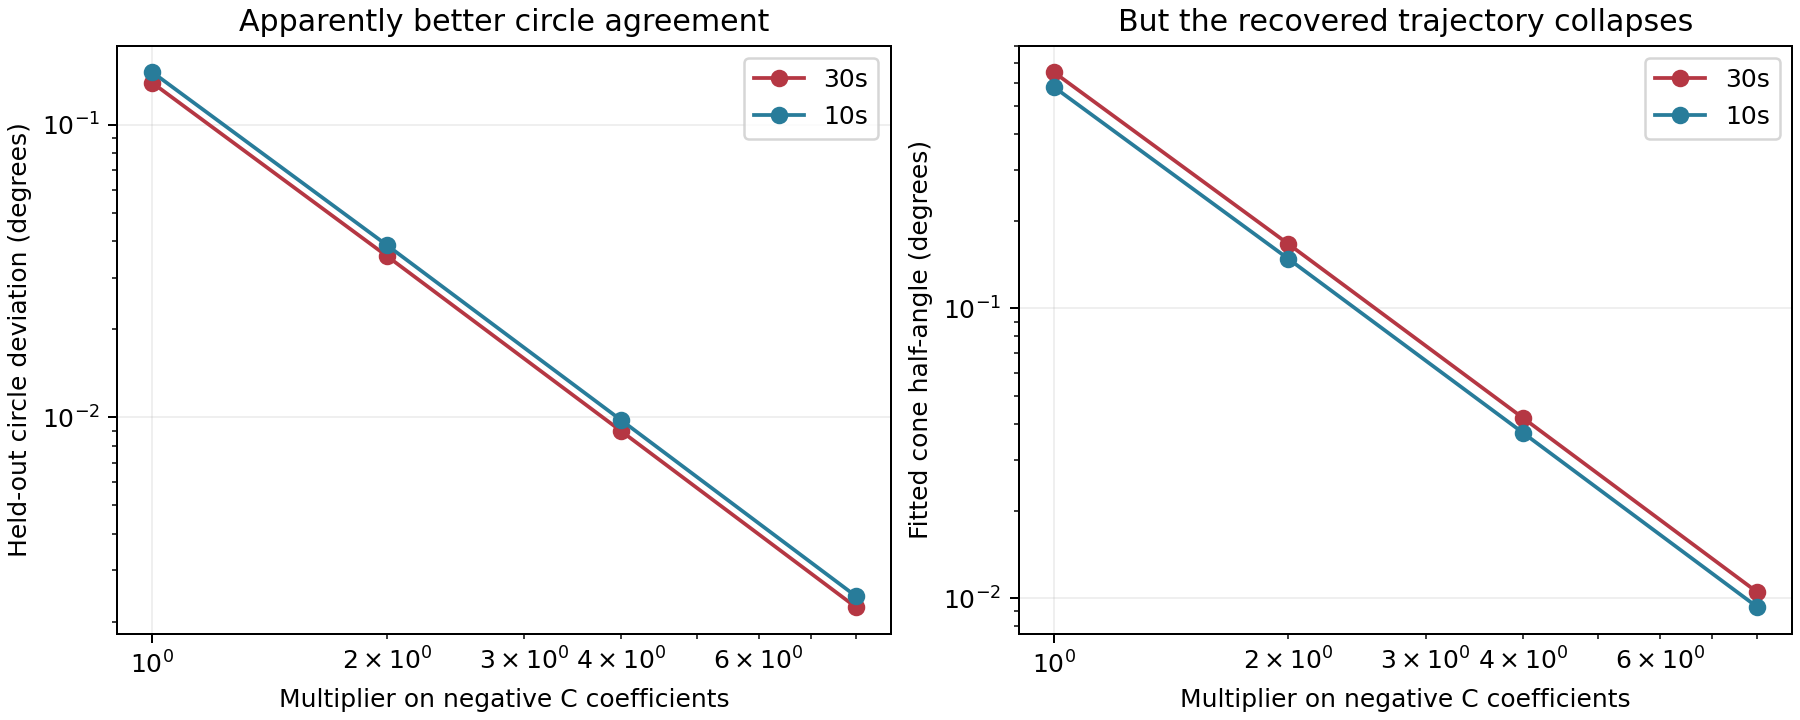
\includegraphics[width=\linewidth]{collapse.png}

The corrected pair sums disagree by roughly 11\% of corrected total at 30 s (15\% at 10 s), despite the near-perfect circle. A common-brightness optical signal cannot explain those recovered four channels. This illustrates why circle agreement must retain the information discarded by the two anisotropy ratios. The initial numerical coefficient box was [-5,5]; the scaling test shows that this box merely truncates the collapse, not that it resolves it.
\newpage
{\Large Retaining intensity information in the inverse approach}

A second pilot profiles the plane, projects each recovered direction onto its circle, evaluates the full four-channel model with one fitted brightness scale, and minimizes the original relative-intensity residual. Phase locations are inferred from each observed four-channel vector, not independently adjusted parameters.

\begin{tabular}{llrrrr}\toprule
Window & Inverse reconstruction & Channel RMS & BG/\(T_{\max}\) & Recovered \(\theta\) & Circle RMS\\\midrule
30s & Additive & 0.06448 & 16.3\% & 5.8--84.7$^\circ$ & 7.13$^\circ$ \\
30s & Richard four-C & 0.05982 & --- & 8.2--76.8$^\circ$ & 7.25$^\circ$ \\
30s & Additive + interference & 0.06448 & 16.3\% & 5.8--84.7$^\circ$ & 7.13$^\circ$ \\
10s & Additive & 0.06160 & 17.9\% & 8.1--80.8$^\circ$ & 7.21$^\circ$ \\
10s & Richard four-C & 0.05849 & --- & 7.6--71.9$^\circ$ & 6.64$^\circ$ \\
10s & Additive + interference & 0.04839 & 20.1\% & 10.5--79.5$^\circ$ & 8.80$^\circ$ \\
\bottomrule\end{tabular}

\textbf{Interpretation limits.} These are conditional held-out reconstruction scores: background, plane and brightness are trained on training cycles, but each held-out vector supplies its own recovered direction and hence phase location. They are not the same prediction test as evaluating a fixed curve at predetermined held-out bin indices. The 30 s complex result retains the nested additive solution because the searches did not improve its feasible training cost; it is not a separately converged complex optimum.

The strict pilot requires nonnegative corrected roots, anisotropy below the Fourkas maximum, and a closed continuous lift in one hemisphere. It retains acquisition order; no nearest-point permutation is allowed. The inferred phase is checked for backtracking; selected reconstruction examples show none or only small fluctuations. Hemisphere-crossing branches are not globally searched. These searches do not prove that a more complete inverse treatment cannot work.

The first unconstrained trials included nonclosing lifted trajectories and out-of-domain points. They are retained as diagnostic failures, not accepted angle corrections. Some circle-only complex solutions were feasible on training data but exceeded the physical anisotropy range on held-out data; these cannot be interpreted by clipping theta. Strict reconstructed examples above have valid held-out inversions.

\textbf{Why branch handling matters.} Fourkas inversion determines folded theta and phi modulo pi. A collection of individually admissible points is not automatically a continuous closed physical trajectory. A cone crossing the equator also folds when represented only on the upper hemisphere. Eliminating explicit cone parameters does not eliminate these geometric decisions.

\textbf{Recommended interpretation.} Keep the equal-arc fits as the controlled comparison. The bounded interference extension tested here does not resolve the shape mismatch. The inverse route is useful as a diagnostic, but a raw spherical-circle objective is demonstrably insufficient: it must enforce four-channel optical consistency, brightness and branch continuity, or explicitly incorporate their measurement uncertainty. Neither route establishes absolute angle truth from these data.

Scripts, caches and numerical details are in model\_comparison/inverse\_circle/. No commit or push.
\end{document}
